\section{Part: Satellite Tracking }\label{sec:q2}    

\subsection{}

\indent Dry tropospheric error depends on pressure at MSL. This means that the height above MSL, at which the measurement is being taken, needs to be accounted for. Moreover, path length proportional to $1/\cos Z$, where $Z$ is zenith angle, has to be taken into consideration.\\
\indent Wet tropospheric error is dependent on humidity (do not confuse with water!) contained in the atmosphere. It is latitude- and (highly) time-dependent. On average, the greatest WVP (water vapor path) occur in the daytime on low latitudes. The remedy for this problem is to install WVR (water vapor radiometer) onboard, which would, upon measuring WVP, include precise corrections in the data sent to the receiver. \\
\indent Ionospheric effects (refraction and dispersion) might be taken care of by means of double-frequency measurements, presented below. In this manner, the range and the TEC (total electron content parameter - related to $\alpha$) might be obtained.
\begin{figure}[H]
		\centering
		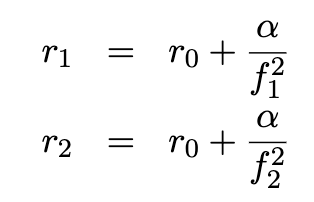
\includegraphics[width=0.15\linewidth]{eq3.png}
\end{figure}

\subsection{}
i) Doppler effect, atmospheric errors (twice - upwards and downwards)\\
ii) \\1. Correct for downward atmospheric errors \\2. Correct for Doppler effect \\3. Mitigate upward atmospheric errors

\subsection{}
i) The primary acceleration that is included in the model is obviously the gravitational acceleration
\begin{center}
	$\ddot{\bar{x}} = -\mu/r^3\:\bar{x}$
\end{center}
apart from which, also perturbations (gravitational pull from other bodies, drag, solar radiation) might be included in the model.\\
ii) Gravitational, solar wind, gravitational perturbations (distant bodies, other satellites etc.), drag, solar wind\\
iii) Gravity field (U), position, velocity, clock corrections, atmospheric parameters (e.g. TEC)\\

\subsection{}
The rotation of the Earth is given by $\bar{\omega} = [0,0,\omega]^T$. Therefore, translation between the frames is
\begin{center}
	$\bar{x}_F = \bar{T}+R_3(\omega \Delta t)\bar{x}_I$
\end{center}
where F signifies the fixed frame values, I - inertial ones, T is the linear translation (null in this case, because the frames have the same origin - center of Earth) and $R_3$ is the rotation matrix around 3rd axis (z).
\begin{center}
	$R_3(\omega \Delta t)
	    \begin{bmatrix}
	    
	        \cos (\omega \Delta t) & \sin (\omega \Delta t) & 0\\[6pt]
	        
	        - \sin (\omega \Delta t) & \cos (\omega \Delta t) & 0\\[6pt]
	        
	        0 & 0 & 1
	        
	        
	    
	    \end{bmatrix}$
\end{center}

\subsection{}

\indent Gravity field is different for all mentioned cases, which translates to different time experienced by atomic clocks. According to the relativity theory, time experienced by the observer (a clock in this case) depends on the gravity field (or velocity), at which the observer is located.












